\section{Machine Learning Workloads} \label{sec-ml-workloads}
We define a machine learning workload as a series of exploratory data analysis steps followed by one or multiple model building steps to solve a machine learning \textit{task}.
We define a machine learning task as designing a set of data transformation steps and a machine learning model, to transform the training data and train a machine learning model, where the goal is to maximize (or minimize) a quality metric (or an error metric) on an evaluation dataset.
For example, in the \textit{Titanic: Machine Learning from Disaster} competition in Kaggle\footnote{https://www.kaggle.com/c/titanic}, the task is to create a machine learning pipeline and train a classification model on the Titanic training dataset that can predict if a traveler survived the Titanic disaster, with the goal of maximizing the prediction accuracy on a separate test dataset.
%Typically users analyze the data by first performing different transformations to gain insight into the data.
%Then, based on these analyses, they apply the right set of transformations to the data to train one or multiple models on the transformed training data.
%Therefore, machine learning workloads typically consist of both interactive (exploratory analysis) and long-running processes (hyperparameter tuning and model training).
%Using the experiment database, we can speed up the execution of the machine learning workloads.
%By analyzing the experiment database, we can extract the common transformations on data and materialize them.
%Thus, during the interactive exploratory analysis, we first analyze the workload to look for reuse opportunities and return the materialized data when possible.
%Moreover, using the experiment database, we provide the users with already trained models or promising hyperparameters which decreases the execution time of the hyperparameter search and model training.

The Kaggle platform allows users to submit their workloads in scripts (called notebooks or kernels) to the Kaggle platform.
Users can view, copy (fork) the notebooks, modify them, and submit them for evaluation.
Figure \ref{fig-titanic-script-hierarchy} shows the most popular notebooks and their relationship.
For example, in the Notebook "Best Working Classifier", the author cites the Notebook "Exploring Survival" as his/her inspiration.
The numbers show how many times each script is forked.
The top most-voted notebooks for the Titanic competition have been forked a total of 44,434 times.
This demonstrates that many of the workloads share similar operations.
By utilizing an experiment database, we plan to optimize new workload by automatically removing redundant operations, speed up the model training, and perform more efficient hyperparameter tuning.
\begin{figure}
\centering
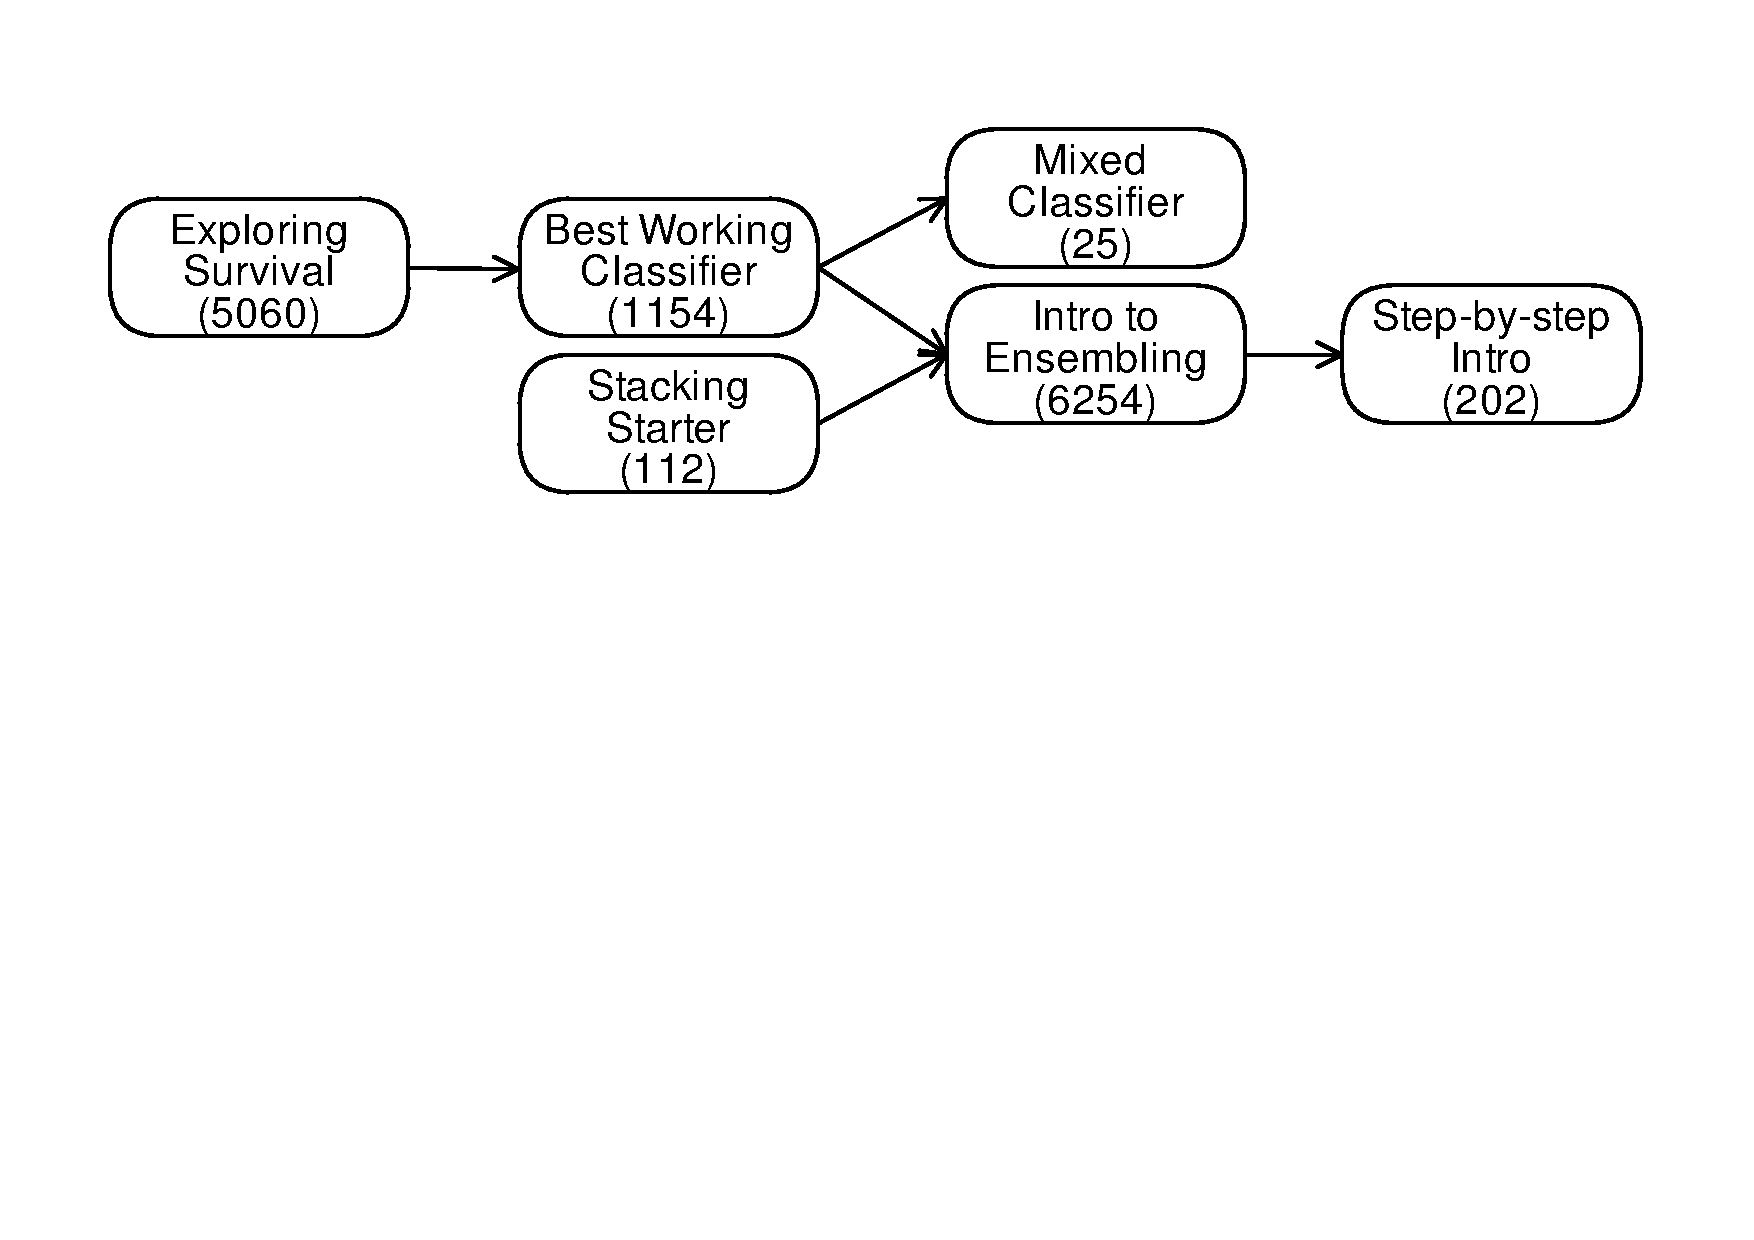
\includegraphics[width=\columnwidth]{../images/kaggle-titanic-scripts-graph}
\caption{The fork hierarchy of some of the popular notebooks in Kaggle's Titanic competition}
\label{fig-titanic-script-hierarchy}
\end{figure}

In order to apply the materialization optimization, we first define the characteristics of the machine learning workloads.
Then, we specify how to detect reuse opportunities from the experiment database.

\subsection{Operations in Machine Learning Workloads}
We assume the main units of work are dataframe like objects that contain one or many columns, where all the data items in one column are of one data type.
We divide the operations in the ML workloads into 3 categories.
\begin{table}
\centering
\begin{tabular}{ll}
\hline
	   Feature Extraction & Feature Selection\\ \hline
        feature hasher & variance threshold  \\
        one hot encoding & select k best \\
        count vectorizer& select percentile \\ 
        tfidf transformer & recursive feature elimination \\
        hashing vectorizer & select from model \\
        extract\_patch\_2d &  \\
        \hline
\end{tabular}
\caption{List of feature extraction and feature selection operations}\label{feature-engineering-operations}
\end{table}

\textbf{1. Data transformation and Feature engineering:}
\begin{itemize}
\item simple data transformations
\item feature selection operations
\item feature extraction operations
\item user-defined feature engineering operations
\end{itemize}
Table \ref{feature-engineering-operations} shows the list common feature extraction and feature selection operations.

\textbf{2. Model Training: }
\begin{itemize}
\item model training operation that applies a training algorithm to a dataset
%\item common aggregation operations (such as mean, max, min, and percentile)
%\item user-defined aggregation operations 
\end{itemize}

Each model building operation results in objects that can either be used in other feature engineering operations (applying PCA to data or categorizing a column based on values in percentile aggregate) or can be a complete machine learning model that can be used to make predictions on unseen data.

\textbf{3. Hyperparameter Tuning:}
The goal of hyperparameter tuning operations are to find the models with the highest quality metric.
A hyperparameter tuning operation is defined by a budget and a search method.
The budget specifies how many models the operation should train and the search method specifies the what search strategy should be incorporated.
We limit our focus to popular search methods, namely, grid search, random search, and Bayesian hyperparameter search.

\subsection{Graph Representation}\label{sub-graph-construction}
To efficiently apply our optimizations, we utilize a graph data structure (called the experiment graph) to store the meta-data and logs of the machine learning workloads.
Let $\mathcal{V}=\{v_i\}, i = 1, \cdots, n$ be a collection of artifacts that exist in the experiment database.
Each artifact is either a raw dataset, a pre-processed dataset resulting from a feature engineering operation, or a model resulting from a model training operation.
Let $\mathcal{E}=\{e_i\}, i = 1, \cdots, m$ be a collection of executed operations that exist in the experiment database.
A directed edge $e$ from $v_i$ to $v_j$ in $\mathcal{G}(\mathcal{V},\mathcal{E})$ indicates that the artifact $v_j$ is (fully or partially) derived from the artifact $v_i$ by applying the operation in $e$.
Every vertex $v$ has the attribute $\langle s \rangle$ (accessed by $v.s$), which represents the storage size of artifact when materialized.
Every edge $e$ has the attributes $\langle f, t\rangle$ (accessed by $e.f$ and $e.t$), where $f$ represents the frequency of the operation (the number of times the operation has been executed) and $t$ represents the average run-time (in seconds) of the operation.
Furthermore, each vertex contains meta-data about the artifacts (such as the name and type of the columns for datasets and name, size, value of parameters and hyperparameters, and loss value of the models) and each edge contains the meta-data about the operation (such as the function name, training algorithm, hyperparameters, and in some cases even the source code of the operation).
When a new machine learning workload is executed, we extend the graph to capture the new operations and artifacts.
If an operation already exists in the graph, we update the frequency and average run-time attributes.
Otherwise, we add a new edge and vertex to the experiment graph, representing the new operation and the artifact.
Figure \ref{fig-experiment-graph} and  shows an example graph constructed from the code in Listing \ref{listing-experiment-graph} based on the Avito demand prediction challenge\footnote{https://www.kaggle.com/c/avito-demand-prediction/}.
To uniquely identify an edge, we utilize a hash function that receives as input the operation and hyperparameters.

\begin{lstlisting}[language=Python, caption=Example script,captionpos=b,label = {listing-experiment-graph}]
import numpy as np
import pandas as pd

from sklearn import svm
from sklearn.feature_selection import SelectKBest
from sklearn.feature_extraction.text import CountVectorizer

train = pd.read_csv('../input/train.csv') 
print train.columns # [ad_desc,ts,u_id,price,y]
vectorizer = CountVectorizer()
count_vectorized = vectorizer.fit_transform(train['ad_desc'])
selector =  SelectKBest(k=2)
top_features = selector.fit_transform(train[['ts','u_id','price']], 
				      train['y'])
X = pd.concat([count_vectorized,top_features], axis = 1)
model = svm.SVC()
model.fit(X, train['y'])
\end{lstlisting}

\begin{figure}
\begin{subfigure}[b]{0.4\linewidth}
\centering
\documentclass{standalone}
\usepackage{tikz}
\usetikzlibrary{graphdrawing, graphs, quotes, positioning,arrows, backgrounds, math, calc, shapes, positioning}
\usegdlibrary{trees}
\begin{document}
\begin{tikzpicture}
%\draw[help lines]  (-2,0) grid (6,6);
\tikzstyle{every node}=[inner sep=0.02cm]
\node (train) [ellipse, draw] at (3,6) {\normalsize $train$};
% layer 1
\node (ad) [ellipse, draw]  at (0,5.5){\normalsize $ad\_desc$};
\node (forselection) [ellipse, draw] at (3.5,5.4) {\normalsize $t\_subset$};
\node (y) [ellipse, draw] at (5.5, 5.5){\normalsize $y$};
% layer 2
\node (cv) [ellipse, draw] at (1,4.9) {\normalsize $cnt\_vect$};
\node(sk) [ellipse, draw]  at (4,4.6){\normalsize $top\_feats$};
% layer 3
%\node (merged1) [circle, draw] at (1.5, 3.5) {$v_6$};
\node (cvsk) [ellipse, draw] at (3.7,3.8) {\normalsize$X$};
% layer 4
%\node(merged2) [circle, draw] at (3, 2.8) {$v_8$};
% layer 5
\node(model) [ellipse, draw, fill=green!20] at (4.9, 3.5)  {$model$};

\graph [grow down,edge quotes ={inner sep=1pt}, edges ={thick},radius=.2cm, nodes={circle, draw,font =\small}]{
(train) [label=train]
->  (ad)
-> (cv)
%-> [anchor=east,align=center,"m"](merged1) 
->(cvsk) 
%-> [anchor=south, align=center,"m"](merged2) ;
-> (model);

(train) 
-> (forselection)
-> (sk)
-> (cvsk) ;

(train) 
->    (y)
%-> [anchor=west, align=center,"m"](merged2) 
->  (model);
};
\end{tikzpicture}
\end{document}
\caption{}
\end{subfigure}%
\begin{subfigure}[b]{0.6\linewidth}
\begin{tabular}{lcl}
\hline
operation & label &  hash \\
\hline
project(ad..) & $\langle 1, 2\rangle$ &p1 \\
project(ts, ..) & $\langle 1, 6\rangle$ & p2\\
project(y) & $\langle 1, 2\rangle$ & p3\\
vectorizer.f\_t & $\langle 1, 40\rangle$ & v1 \\
selector.f\_t & $\langle 1, 60\rangle$ & s1 \\
concat & $\langle 1, 10\rangle$ & c1 \\
merge & $\langle 1, 0 \rangle$ & m\\
model.fit & $\langle 1, 100\rangle$ & f1\\

\end{tabular}
\caption{}
\end{subfigure}
\caption{Experiment graph constructed from the Listing \ref{listing-experiment-graph} (a) and the hash of the operations in the scripts (b)}
\label{fig-experiment-graph}
\end{figure}
Table \ref{fig-experiment-graph}b shows both the label of every edge operation (frequency and time in seconds) and the (arbitrary) hash of the operations and their hyperparameters.

In order to represent operations that process multiple input artifacts (e.g., concat and model.fit operations in Listing \ref{listing-experiment-graph}), we proceed as follows.
First, we merge the vertices representing the artifacts into a single vertex using merge operator.
The merge operator is a logical operator which does not incur a cost (run-time of 0 seconds).
Then, we draw an edge from the merged vertex which represents the actual operation.
For example, in Figure \ref{fig-experiment-graph}, before applying the concatenation operation, we merge $v_4$ and $v_5$ into $v_6$, then we apply the concatenation operation (c1).
This is a critical step for our materialization algorithm in Section \ref{subsec-materialization} and our optimization strategies discussed in Sections \ref{sec-reuse-and-warmstarting} and \ref{sec-hyperparam-optimization}.

It is important to note that based our definition of a task in Section \ref{sec-introduction} if the experiment database contains meta-data about multiple tasks, the constructed graph will contain one connected component for every task.
In the next sections, we assume that the experiment database contains information about 1 task, although, all the methods described can be applied to multiple tasks as well.

\subsection{Materialization of the Experiment Graph}\label{subsec-materialization}
Depending on the number of the executed workloads, the generated artifacts may require a large amount of storage space.
For example, in the Home Credit Default Risk Kaggle competition, one of the popular scripts that analyzes a dataset of 150 MB, generates up to 10 GB of artifacts.
\todo[inline]{10 GB is a rough estimate, I need to finish the code to accurately calculate the number}
Therefore, materializing every artifact is not feasible.
In this section, we discuss our algorithm for materializing a subset of the artifacts under limited storage.
The goal of the algorithm is to materialize the artifacts that result in the lowest weighted recreation cost while ensuring the total size of the materialized artifacts does not exceed the storage capacity.
We define the weighted recreation cost of the graph $\mathcal{G}$, given the set of materialized vertices $\mathcal{MV}$ as 
\[
weighted\_recreation\_cost(\mathcal{G}, \mathcal{MV}) =  \sum\limits_{e \in \{e' \in \mathcal{E}  \lvert dest(e') \notin \mathcal{MV}\}}  e.f \times e.t
\]
where $dest(e)$ represent the destination vertex of the edge $e$.
The weighted recreation cost indicates how much time do we need to spend to execute all the operations in the graph, since the beginning of time.
For un-materialized artifacts, we must consider the frequency of the operations that produce the artifact.
For example, in Figure \ref{fig-experiment-graph}, if we do not materialize $v_4$ and the operation \textit{count\_vectorizer} has a frequency of 10, we must consider all 10 executions of the operation when computing the weighted cost.
Whereas, if $v_4$ is materialized, the \textit{count\_vectorizer} operation has no impact on the weighted recreation cost.
We propose a local greedy algorithm to the problem.
%\todo[inline]{show that it is NP hard and cite \cite{bhattacherjee2015principles} and state the differences in their work and solution and ours}
%Bhattacherjee et al. \cite{bhattacherjee2015principles} tackle a similar problem and prove that the problem is NP-hard.
%They provide a greedy solution for the problem as well.
%However, there differences in both the use cases and problem formulation that make their solution not feasible in our case.

\begin{algorithm}[h]
\caption{Materialization of Artifacts}\label{algorithm-materialization}
\begin{algorithmic}[1]
\Require  $\mathcal{G(V,E)}=$ experiment graph, $\mathcal{B}=$ storage limit
\Ensure $\mathcal{MV}=$ set of materialized artifacts
\State $T=v_0.size$, $\mathcal{MV} =\{v_0\}$
\Do 
	\State $\mathcal{CV} = \{v \in \mathcal{V} \lvert v \notin \mathcal{MV}, T + v.s \leq \mathcal{B}\}$
	\State $v^* = \argmax\limits_{v \in \mathcal{CV}} \tfrac{\rho(\mathcal{G}, v)}{v.s}$
	\State $\mathcal{MV} = \mathcal{MV} \cup \{v^*\}$
	\State $T = T + v^*.size$
\DoWhile{$\mathcal{CV} \neq \emptyset$}
\end{algorithmic}
\end{algorithm}
Algorithm \ref{algorithm-materialization} shows the details of our method for selecting the vertices to materialize.
First, we start by initializing the materialized vertices set ($\mathcal{MV}$) to contain the root artifact ($v_0$) which represents the raw dataset.
This is essential as many of the feature engineering and model building operations are not invertible.
As a result, we cannot reconstruct the raw dataset if it is not materialized.
Then, while the storage limit is not reached, we materialize vertices with the maximum value of weighted recreation cost over size.
We compute the weighted recreation cost ($\rho$) of the vertex $v$ as, 
\[
\rho(\mathcal{G}, v) = \alpha(\mathcal{G}, v) \times \sum\limits_{e \in path(\mathcal{G}, v_0, v)}  e.t
\]
where $\alpha(\mathcal{G}, v)$ represents the access frequency of the vertex $v$ which is the same as frequency of the edge (or any of the edges in case of merge operation) connected to $v$.
The set $path(\mathcal{G}, v_0, v)$ represents the set of all edges from the root node to the vertex $v$. 
For example, in Figure \ref{fig-materialization-example}, the recreation cost of $v_4$ is $3 \times (0 + 0 + 25 + 10 + 10) = 135$.
The ratio of the weighted recreation cost over size has the unit second per megabyte.
For example, the ratio 10 s/mb for an artifact, indicates that we need to spend 10 seconds to recreate 1 megabyte of the artifact.
Figure \ref{fig-materialization-example} shows an example of the materialization process when the storage capacity is 55.
For $v_0$ we do not compute $\rho$ as $v_0$ is always materialized.

\begin{figure}
\begin{subfigure}{0.5\linewidth}
\centering
\begin{tikzpicture}%[background rectangle/.style={fill=olive!45}, show background rectangle]
\tikzstyle{every node}=[inner sep=0.02cm]
\tikzstyle{every label}=[font=\scriptsize]
\tikzstyle{materialized} = [fill=green!25]
%\draw[help lines]  (-2,-3) grid (6,6);
\node(v0)[circle, draw] at (-1,5.5) {$v_0$};
% layer 1
\node(v1)[circle, draw] at (-1.8,4.8){$v_1$};
\node(v2)[circle, draw] at (-0.2,4.8) {$v_2$};
% layer 2
\node(v3)[circle, draw] at (-1.8,3.8) {$v_3$};
\node (v4) [circle, draw] at (-1, 3.2) {$v_4$};
\node(v5)[circle, draw] at (-0.2, 3.8) {$v_5$};
%layer 3
\node(v6)[circle, draw] at (-1.8, 2.5) {$v_6$};
\node(v7)[circle, draw] at (-0.2,2.5) {$v_7$};
\graph [edges ={thick}]{
(v0)
-> [swap,anchor=mid,align=left,font=\scriptsize,"$\langle3,0\rangle$"] (v1)
-> [swap,anchor=mid,font=\scriptsize,"$\langle3,25\rangle$"] (v3)
-> [swap,anchor=mid,font=\scriptsize,"$\langle3,10\rangle$"]  (v4) ;
(v0) 
-> [font=\scriptsize, "$\langle3,0\rangle$"] (v2)
-> [font=\scriptsize,"$\langle2,25\rangle$"] (v5);
(v2) 
-> [swap,anchor=mid,font=\scriptsize,anchor=mid, align=center,"$\langle3,10\rangle$"]   (v4);
(v4)
-> [swap,font=\scriptsize,"$\langle1,60\rangle$"]  (v6) ;
(v4)
-> [font=\scriptsize,"$\langle2,30\rangle$"]  (v7); 
};
%
%\begin{scope}[shift={(5,0)}]
%	\node(v0)[label={$\langle\textbf{10}\rangle$}] [circle, draw] at (-1,5.5) {$v_0$};
%	% layer 1
%	\node(v1)[label=left:$\langle\textbf{8}\rangle$] [circle, draw] at (-1.8,4.8){$v_1$};
%	\node(v2)[label=left:$\langle\textbf{2}\rangle$] [circle, draw] at (-0.2,4.8) {$v_2$};
%	% layer 2
%	\node(v3)[label=left:$\langle\textbf{40}\rangle$] [circle, draw] at (-1.8,3.8) {$v_3$};
%	\node (v4)[label=below:$\langle\textbf{42}\rangle$] [circle, draw] at (-1, 3.2) {$v_4$};
%	\node(v5)[label=right:$\langle\textbf{0.1}\rangle$] [circle, draw] at (-0.2, 3.8) {$v_5$};
%	%layer 3
%	\node(v6)[label=below:$\langle\textbf{2}\rangle$] [circle, draw] at (-1.8, 2.5) {$v_6$};
%	\node(v7)[label=below:$\langle\textbf{2}\rangle$] [circle, draw] at (-0.2,2.5) {$v_7$};
%	\graph [edges ={thick}]{
%	(v0)
%	-> [swap,anchor=mid,align=left,font=\scriptsize,"$\langle3,0\rangle$"] (v1)
%	-> [swap,anchor=mid,font=\scriptsize,"$\langle3,20\rangle$"] (v3)
%	-> [swap,anchor=mid,font=\scriptsize,"$\langle3,1\rangle$"]  (v4) ;
%	(v0) 
%	-> [font=\scriptsize, "$\langle3,0\rangle$"] (v2)
%	-> [font=\scriptsize,"$\langle2,2\rangle$"] (v5);
%	(v2) 
%	-> [swap,anchor=mid,font=\scriptsize,anchor=mid, align=center,"$\langle3,1\rangle$"]   (v4);
%	(v4)
%	-> [swap,font=\scriptsize,"$\langle1,60\rangle$"]  (v6) ;
%	(v4)
%	-> [font=\scriptsize,"$\langle2,40\rangle$"]  (v7); 
%	};
%\end{scope}
\end{tikzpicture}
\caption{Original Graph}
\label{fig-materialization-example}
\end{subfigure}%
\begin{subfigure}{0.5\linewidth}
\centering
\begin{tikzpicture}%[background rectangle/.style={fill=olive!45}, show background rectangle]
\tikzstyle{every node}=[inner sep=0.02cm]
\tikzstyle{every label}=[font=\scriptsize]
\tikzstyle{materialized} = [fill=green!25]

\node(v0)[materialized][circle, draw] at (-1,5.5) {$v_0$};
% layer 1
\node(v1)[circle, draw] at (-1.8,4.8){$v_1$};
\node(v2)[materialized][circle, draw] at (-0.2,4.8) {$v_2$};
% layer 2
\node(v3)[circle, draw] at (-1.8,4.0) {$v_3$};
\node (v4) [circle, draw] at (-1, 3.5) {$v_4$};
\node(v5)[materialized][circle, draw] at (-0.2, 4.0) {$v_5$};
%layer 3
\node(v6)[materialized][circle, draw] at (-1, 2.7) {$v_6$};
%layer 4
\node(v7)[materialized][circle, draw] at (-1.8, 2.0) {$v_7$};
\node(v8)[materialized][circle, draw] at (-0.2, 2.0) {$v_8$};
\graph [edges ={thick}]{
(v0)
-> [swap,anchor=mid,align=left,font=\scriptsize,"$\langle3,1\rangle$"] (v1)
-> [swap,anchor=mid,font=\scriptsize,"$\langle3,25\rangle$"] (v3)
-> [swap,anchor=mid,font=\scriptsize,"$\langle3,0\rangle$"]  (v4) 
-> [anchor=mid,align=right,font=\scriptsize,"$\langle3,20\rangle$"] (v6); 
(v0) 
-> [font=\scriptsize, "$\langle3,1\rangle$"] (v2)
-> [font=\scriptsize,"$\langle2,25\rangle$"] (v5);
(v2) 
-> [swap,font=\scriptsize,align=right,"$\langle3,0\rangle$"]   (v4);
(v6)
-> [swap,font=\scriptsize,"$\langle1,60\rangle$"]  (v7) ;
(v6)
-> [font=\scriptsize,"$\langle2,30\rangle$"]  (v8); 
};

\end{tikzpicture}
\caption{Materialized Graph}
\label{fig-materialization-example}
\end{subfigure}
\begin{subfigure}{\linewidth}
\setlength\tabcolsep{3.5pt} % This is to ensure the table does not go out of bound
\begin{tabular}{l | | >{\bfseries}r | r  |>{\bfseries}r | r | r | >{\bfseries}r | >{\bfseries}r | >{\bfseries}r |>{\bfseries}r }
\hline
\textbf{vertex} & $\boldsymbol{v_0}$ & $v_1$ & $v_2$ & $v_3$ & $\boldsymbol{v_4}$ & $\boldsymbol{v_5}$ & $\boldsymbol{v_6}$ & $\boldsymbol{v_7}$ &$\boldsymbol{v_8}$ \\
\hline
\textbf{size (MB)}    & 10 & 8 & 2 & 40 & 42 & 1 & 30 & 2   & 3        \\
\textbf{$\boldsymbol{\rho}$ (s)} & ---   & 3 & 3 & 78 & 81 & 52 & 141 & 107 & 154	  \\
\textbf{ratio}& ---   & 0.37 & 1.5 & 1.95 & 1.93 & 52 & 4.7 & 53.5 & 51.3	\\
\hline
\end{tabular}
\caption{List of vertices, their sizes, recreation costs, and the cost over size ratio (Bold vertices are materialized).}
\end{subfigure}
\caption{Artifact materialization based on Algorithm \ref{algorithm-materialization} when storage capacity is 55 (MB)}
\end{figure}

\subsubsection{The Effect of Model Quality on the Materialization Decision}
Since the goal of all the workloads in the experiment graph is to solve the same task (as described in \ref{sec-introduction}), all the machine learning models will be evaluated using the same quality metric.
Therefore, we can utilize the quality of the model in the materialization algorithm.
We propose a simple method for utilizing the model quality in the materialization decision algorithm.
We start by adding a new attribute $q$ to every edge.
The new attribute is computed as follows.
If the edge $e$ belongs to no path that leads to a predictive model, we assign $q$ to the average quality of all the predictive models in the experiment graph.
If $e$ belongs to only one path that leads to a predictive model, then we assign $q$ to the quality of the model.
If $e$ belongs to multiple paths that lead to different predictive models, we assign $q$ to the quality of the model with the maximum quality among all the models.
After computing $q$, we include it in the computation of $\rho$, by multiplying $e.q$ by $e.t$ in the summation. 

\subsection{Optimization Workflow}
Figure \ref{fig-system-workflow} shows the workflow of our system.
First, we transform the workload script into its graph representation.
Then we utilize the experiment graph to optimize the workload (using the techniques in Sections \ref{sec-reuse-and-warmstarting} and \ref{sec-hyperparam-optimization}).
This results in a new workload graph which depending on the types of optimizations may have a fewer number of operations (\textit{reuse optimization}, faster operations (\textit{warmstarting}), or operation configurations that lead to higher quality machine learning models (\textit{improved hyperparameter tuning}).
\begin{figure}
\centering
\newcommand*{\connectorH}[4][]{
  \draw[#1, thickarrow] (#3) -| ($(#3) !#2! (#4)$) |- (#4);
}
\begin{tikzpicture}%[background rectangle/.style={fill=olive!45}, show background rectangle]
\tikzstyle{thickarrow}=[line width=0.5mm,draw=gray!128,-triangle 45,postaction={draw, line width=1mm, shorten >=1mm, -}]
\tikzstyle{every label}=[font=\scriptsize]
\tikzstyle{graphnode} = [inner sep=0.04cm, fill=black!255]
\tikzstyle{dummynode} = [inner sep=0.04cm, fill=black!0, line width=0mm]
%\draw[step=1cm,gray,very thin] (-2,0) grid (6,4);

%dummy nodes
\node(dn0) at (0.7, 3) {};
\node(dn1) at (1.7, 3) {};
\node(dn2) at (4.1, 3) {};
\node(dn3) at (5.1, 3) {};
\node(dn4) [inner sep=0.01cm] at (0.3,3) {};

\tikzmath{\x = -1.3; \y =3; }
\node(ws0)[rectangle, text width =1.2cm,minimum width=1.2cm, minimum height=2cm,align=center, draw] at (\x,\y) {workload script};

\tikzmath{\x = .7; \y =3.65; }
\node(wg0)[graphnode,circle, draw] at (\x,\y) {};
\node(wg1)[graphnode,circle, draw] at (\x-0.2,\y-0.4){};
\node(wg2)[graphnode,circle, draw] at (\x-0.2,\y-0.8) {};
\node(wg3)[graphnode,circle, draw] at (\x-0.4,\y-1.2) {};
\node [text width =1.5cm, align=center] at (0.5,2) {original workload};

\tikzmath{\x = 2.9; \y =3.6; }
\node(eg0)[graphnode,circle, draw] at (\x,\y) {};
\node(eg1)[graphnode,circle, draw] at (\x-0.5,\y-0.4) {};
\node(eg2)[graphnode,circle, draw] at (\x,\y-0.4) {};
\node(eg3)[graphnode,circle, draw] at (\x+0.5,\y-0.4) {};
\node(eg4)[graphnode,circle, draw] at (\x -0.75,\y-0.8) {};
\node(eg5)[graphnode,circle, draw] at (\x-0.25,\y-.8){};
\node(eg6)[graphnode,circle, draw] at (\x + 0.25,\y-.8) {};
\node(eg7)[graphnode,circle, draw] at (\x+.75,\y-.8) {};
\node(eg8)[graphnode,circle, draw] at (\x-1,\y-1.2) {};
\node(eg9)[graphnode,circle, draw] at (\x -0.5,\y-1.2) {};
\node(eg10)[graphnode,circle, draw] at (\x,\y-1.2){};
\node(eg11)[graphnode,circle, draw] at (\x + 0.5,\y-1.2) {};
\node(eg12)[graphnode,circle, draw] at (\x+1,\y-1.2) {};
\node [text width =1.5cm, align=center] at (2.9,1.6) {Experiment graph};

\tikzmath{\x = 5.5; \y =3.4; }
\node(og0)[graphnode,circle, draw] at (\x,\y) {};
\node(og1)[graphnode,circle, draw] at (\x-0.2,\y-0.4){};
\node(og2)[graphnode,circle, draw] at (\x-0.4,\y-0.8) {};
\node [text width =1.5cm, align=center] at (5.3,2) {optimized workload};
\draw[dashed, thick] (1.7,2.1) rectangle (4.1,3.9);
\graph []{
(ws0) -> [>=stealth, line width=0.7mm] (dn4);
(wg0) -> (wg1) -> (wg2) -> (wg3);
(eg0) -> (eg1) -> (eg4) -> (eg8);
(eg0) -> (eg2) -> (eg5) -> (eg9);
(eg5) -> (eg10);
(eg0) -> (eg3) -> (eg7) -> (eg12);
(eg3) -> (eg6) -> (eg11);
(eg2) -> (eg6);
(og0) -> (og1) -> (og2);
(dn0) -> [>=stealth, line width=0.7mm] (dn1);
(dn2) -> [>=stealth, line width=0.7mm](dn3);
};
\end{tikzpicture}
\caption{System workflow}
\label{fig-system-workflow}
\end{figure}
%\subsection{Artifacts Unique Identifiers}
%To uniquely identify artifacts, we utilize a similar method to \textit{Trie}\footnote{https://en.wikipedia.org/wiki/Trie}.
%As a result, we can uniquely identify each artifact by performing a walk starting from the root node and concatenate the hash of every operation and its hyperparameters to name a vertex.
%For merge operations (two edges entering a vertex), we  
